% Preamble template for Tufte-style lecture notes.
% Do not compile this file directly; compile the main notes file instead.
\documentclass{tufte-handout}

\usepackage{ntheorem}
\usepackage{graphicx}
\usepackage{amsmath}
\usepackage{amssymb}
\usepackage{hyperref}
\usepackage{epigraph}
\usepackage{booktabs}
\theoremstyle{break}
% \usepackage[
% bibencoding=utf8,% .bib file encoding
% maxbibnames=3, % otherwise et al
% minbibnames=1, % otherwise et al
% backend=biber,%
% sortlocale=en_US,%
% style=apa,% or authoryear
% % apabackref=false, % backreferences
% natbib=true,% for citet/citep, but this is for backward compatibility
% uniquename=false,%
% url=true,%
% sortcites=false,
% doi=true,%
% eprint=true%
% ]{biblatex}
% \addbibresource{lecture_note_bib.bib}

\hypersetup{
  colorlinks,
  urlcolor = blue,
  pdfauthor={Paul Goldsmith-Pinkham}
  pdfkeywords={econometrics}
  pdftitle={Lecture Notes for Applied Empirical Methods}
  pdfpagemode=UseNone
}
\newtheorem{ruleN}{Rule}
\newtheorem{thmN}{Theorem}
\newtheorem{assN}{Assumption}
\newtheorem{defN}{Definition}
\newtheorem{exmp}{Example}
\newtheorem{cmt}{Comment}
\newtheorem{proof}{Proof}

\newcommand{\continuation}{??}
\newtheorem*{excont}{Example \continuation}
\newenvironment{continueexample}[1]
 {\renewcommand{\continuation}{\ref{#1}}\excont[continued]}
 {\endexcont}
\newcommand{\bY}{\mathbf{Y}}
\newcommand{\bX}{\mathbf{X}}
\newcommand{\bD}{\mathbf{D}}
\newcommand{\E}{\mathbb{E}}

\newcommand\independent{\protect\mathpalette{\protect\independenT}{\perp}}
\def\independenT#1#2{\mathrel{\rlap{$#1#2$}\mkern2mu{#1#2}}}
\DeclareMathOperator{\Supp}{Supp}

\usepackage{cleveref}
\crefname{appsec}{appendix}{appendices}
\crefname{appsubsec}{appendix}{appendices}
\crefname{assumption}{assumption}{assumptions}
\crefname{equation}{equation}{equations}
\crefname{exmp}{example}{examples}
\crefname{assN}{assumption}{assumptions}
\crefname{cmt}{comment}{comments}
\crefname{defN}{definition}{definitions}

\usepackage[nolist]{acronym}
\begin{acronym}
  \acro{CI}{confidence interval}%
  \acro{OLS}{ordinary least squares}%
  \acro{CLT}{central limit theorem}%
  \acro{IV}{instrumental variables}%
  \acro{ATE}{average treatment effect}%
  \acro{RCT}{randomized control trial}%
  \acro{SUTVA}{stable unit treatment value assignment}
  \acro{VAM}{value-added model}%
  \acro{LAN}{locally asymptotically normal}%
  \acro{DiD}{difference-in-differences}%
  \acro{OVB}{omitted variables bias}
  \acro{FWL}{Frisch-Waugh-Lovell}
  \acro{DAG}{directed acyclic graph}
  \acro{PO}{potential outcomes}
\end{acronym}

\def\inprobHIGH{\,{\buildrel p \over \rightarrow}\,} 
\def\inprob{\,{\inprobHIGH}\,} 
\def\indistHIGH{\,{\buildrel d \over \rightarrow}\,} 
\def\indist{\,{\indistHIGH}\,}

\usepackage[many]{tcolorbox} 
\definecolor{main}{HTML}{3F6EA7}      % primary accent
\definecolor{sub}{HTML}{F2F7FD}       % cool background
\definecolor{sub2}{HTML}{FFF5E8}      % warm background
\definecolor{mainline}{HTML}{D3DFEE}  % soft frame for information boxes
\definecolor{warn}{HTML}{C7771B}      % accent for caution boxes
\definecolor{warnline}{HTML}{EAD9C0}  % soft frame for caution boxes

\tcbset{
    enhanced,
    breakable,
    colback = white,
    boxrule = 0.5pt,
    arc = 2pt,
    left = 9pt,
    right = 9pt,
    top = 7pt,
    bottom = 7pt,
    before skip = 0.3cm,
    after skip = 0.45cm
}                           % setting global options for tcolorbox

\newtcolorbox{boxD}{
    colback = sub,
    colframe = mainline,
    borderline west = {2.2pt}{0pt}{main},
    borderline north = {0.6pt}{0pt}{main!25},
    borderline south = {0.6pt}{0pt}{main!15}
}


\newtcolorbox{boxF}{
    colback = sub2,
    colframe = warnline,
    borderline west = {2.2pt}{0pt}{warn},
    borderline north = {0.6pt}{0pt}{warn!25},
    borderline south = {0.6pt}{0pt}{warn!15}
}

\usepackage{colortbl}


\usepackage{tikz}
\usepackage{verbatim}
\usetikzlibrary{positioning}
\usetikzlibrary{snakes}
\usetikzlibrary{calc}
\usetikzlibrary{arrows}
\usetikzlibrary{decorations.markings}
\usetikzlibrary{shapes.misc}
\usetikzlibrary{matrix,shapes,arrows,fit,tikzmark}




\title{S181M116 Derivatives and Alternative Investments: Lecture 2}
\author{Swapnil Singh}
\date{}

\hypersetup{
  pdftitle={S181M116 Derivatives and Alternative Investments: Lecture 2},
  pdfauthor={Swapnil Singh},
  pdfkeywords={derivatives, futures, hedging, basis risk, forward prices, cost of carry, commodities}
}

\setlength{\headheight}{26pt}
\graphicspath{{images/lecture-2/}}

\newcommand{\St}{S_T}
\newcommand{\Szero}{S_0}
\newcommand{\Ft}{F_t}
\newcommand{\Fzero}{F_0}
\newcommand{\K}{K}
\newcommand{\PV}{\mathrm{PV}}
\newcommand{\pnl}{\mathrm{P\&L}}
\newcommand{\Var}{\operatorname{Var}}
\newcommand{\Cov}{\operatorname{Cov}}
\newcommand{\Corr}{\operatorname{Corr}}

\begin{document}
\maketitle

\begin{abstract}
This lecture studies two connected questions. First, how can a firm use futures
contracts to hedge an existing or anticipated exposure? Second, how are forward
and futures prices linked to spot prices, interest rates, income, storage costs,
and convenience yields? The main ideas are short and long hedges, basis risk,
cross hedging, the minimum-variance hedge ratio, stock-index beta hedging,
stack-and-roll hedging, no-arbitrage forward pricing, and commodity cost of
carry.
\end{abstract}

\begin{boxD}
\textbf{Reading.} Hull, Chapters 3 and 5; selected commodity examples from
Chapter 35. The central skill is to translate an economic exposure into a
futures position, then check whether the hedge is exact, approximate, or exposed
to basis risk.
\end{boxD}

\section{Roadmap}

Lecture 1 introduced futures and forwards as contracts. Lecture 2 uses them for
two purposes:
\begin{enumerate}
    \item \textbf{Hedging.} Choose a futures position that offsets a price risk.
    \item \textbf{Pricing.} Use no-arbitrage to connect spot prices, forward
    prices, interest rates, income, and storage benefits.
\end{enumerate}

The two purposes are linked. A hedge works well when futures and spot prices
move together. A pricing formula tells us why they should move together and when
they may diverge.

\begin{boxF}
\textbf{Interpretation.} A hedge does not make a firm ``win'' in all states. It
trades upside for downside protection. If the unhedged position would have gained
from a favorable price move, the hedge will usually give up much of that gain.
\end{boxF}

\section{Basic Hedge Mechanics}

\subsection{The Exposure Comes First}

Before choosing a futures position, identify the firm's exposure:
\begin{itemize}
    \item Will the firm \emph{sell} the asset in the future?
    \item Will the firm \emph{buy} the asset in the future?
    \item Is the exposure to the same asset as the futures contract?
    \item What is the quantity, timing, and currency of the exposure?
\end{itemize}

The hedge should generate gains when the underlying business exposure generates
losses.

\begin{defN}[Short hedge]
A short hedge uses a short futures position. It is natural when the hedger owns,
produces, or expects to receive an asset and will sell it later. The hedge gains
when the futures price falls.
\end{defN}

\begin{defN}[Long hedge]
A long hedge uses a long futures position. It is natural when the hedger expects
to buy an asset later. The hedge gains when the futures price rises.
\end{defN}

\subsection{Short Hedge}

A short hedge is used by a seller who is worried about a price decline. Examples
include:
\begin{itemize}
    \item an oil producer that will sell crude oil in three months;
    \item a farmer that will sell grain after harvest;
    \item a U.S. exporter that will receive euros and later convert them into
    dollars;
    \item a portfolio manager who wants to reduce equity-market exposure.
\end{itemize}

\begin{exmp}[Short hedge for an oil producer]
An oil producer will sell 500,000 barrels of crude oil in three months. The
three-month futures price is USD 78 per barrel. Each futures contract is for
1,000 barrels, so the firm shorts
\[
    N=\frac{500{,}000}{1{,}000}=500
\]
contracts.

Suppose that when the oil is sold, the spot and futures prices are both close to
USD 72. The firm sells physical oil for
\[
    500{,}000\times 72=\$36{,}000{,}000.
\]
The short futures gain is
\[
    500{,}000(78-72)=\$3{,}000{,}000.
\]
Total revenue is
\[
    36{,}000{,}000+3{,}000{,}000=\$39{,}000{,}000,
\]
or USD 78 per barrel.

If instead the final price is USD 84, the firm sells oil for USD 42 million and
loses USD 3 million on futures. Total revenue is again USD 39 million. The hedge
has locked in approximately the futures price.
\end{exmp}

\subsection{Long Hedge}

A long hedge is used by a buyer who is worried about a price increase. Examples
include:
\begin{itemize}
    \item an airline that will buy jet fuel;
    \item a food producer that will buy wheat;
    \item a manufacturer that will buy copper;
    \item an importer that will need foreign currency.
\end{itemize}

\begin{exmp}[Long hedge for a copper buyer]
A manufacturer will need 250,000 pounds of copper in four months. The futures
price is USD 3.70 per pound and each futures contract covers 25,000 pounds. The
firm goes long
\[
    N=\frac{250{,}000}{25{,}000}=10
\]
contracts.

If copper later costs USD 4.10 per pound, the physical purchase costs
\[
    250{,}000\times 4.10=\$1{,}025{,}000.
\]
The long futures gain is
\[
    250{,}000(4.10-3.70)=\$100{,}000.
\]
The net cost is therefore
\[
    1{,}025{,}000-100{,}000=\$925{,}000,
\]
or USD 3.70 per pound.

If the final price is USD 3.40, the firm pays less in the physical market but
loses on futures. The hedge again produces an approximate net purchase price of
USD 3.70 per pound.
\end{exmp}

\subsection{Hedge-and-Forget Versus Dynamic Hedging}

In this lecture, the hedge is usually established at the start and closed at the
end. This is a \emph{hedge-and-forget} strategy. Later in the course, option
hedging requires dynamic rebalancing because option exposures change with the
underlying price, volatility, and time.

\begin{boxD}
\textbf{Rule of thumb.} Linear exposures can often be hedged with a fixed
futures position. Nonlinear exposures usually require dynamic hedging or option
contracts.
\end{boxD}

\section{Why Firms Hedge}

\subsection{Risk Reduction}

Many nonfinancial firms are not in the business of forecasting oil prices,
exchange rates, interest rates, or equity indices. Hedging lets managers focus on
operating decisions rather than market timing.

\begin{exmp}[Budget certainty]
An airline sells tickets months before it buys the fuel needed for those flights.
If fuel prices rise sharply, the revenue from ticket sales may be fixed while
costs increase. A long futures hedge can stabilize the fuel cost per flight and
make route planning more reliable.
\end{exmp}

\subsection{Hedging and Shareholders}

A common argument against corporate hedging is that diversified shareholders can
hedge or diversify risk themselves. This argument is incomplete for several
reasons:
\begin{itemize}
    \item managers usually know more about the firm's exposures than outside
    shareholders;
    \item firms may hedge at lower transaction cost than individuals;
    \item reducing cash-flow volatility can reduce financial distress costs;
    \item stable cash flows can protect investment plans from funding shocks.
\end{itemize}

The strongest case against hedging is when the risk is already naturally passed
through to customers or offset elsewhere in the firm's economics.

\subsection{Hedging and Competitors}

The correct hedge depends on the whole business model. If all firms in an
industry are exposed to the same input cost and output prices adjust with that
input cost, hedging can sometimes increase rather than decrease profit-margin
volatility relative to competitors.

\begin{exmp}[Input cost pass-through]
Suppose jewelry producers buy gold and sell jewelry. If gold prices rise, the
wholesale price of jewelry may also rise. A producer that does not hedge may
maintain a roughly stable margin. A producer that hedges gold purchases may gain
on the hedge when gold rises, but may lose relative to the natural pass-through
when gold falls. The hedge must be evaluated against total firm profit, not only
against the input price.
\end{exmp}

\begin{boxF}
\textbf{Governance issue.} A good hedge can look bad ex post. If a short hedge
loses money because the asset price rose, the underlying business exposure should
have gained. Risk reports should show the combined physical-plus-futures result,
not the futures account in isolation.
\end{boxF}

\section{Basis Risk}

\subsection{The Basis}

The \emph{basis} is the difference between the spot price of the asset being
hedged and the futures price of the contract used for hedging:
\[
    b_t=S_t-F_t.
\]
Some markets define the basis as futures minus spot. In this course note, unless
otherwise stated, we use
\[
    \text{basis}=\text{spot}-\text{futures}.
\]

Basis risk is the risk that the basis at the time the hedge is closed is not the
basis expected when the hedge is initiated.

\begin{marginfigure}
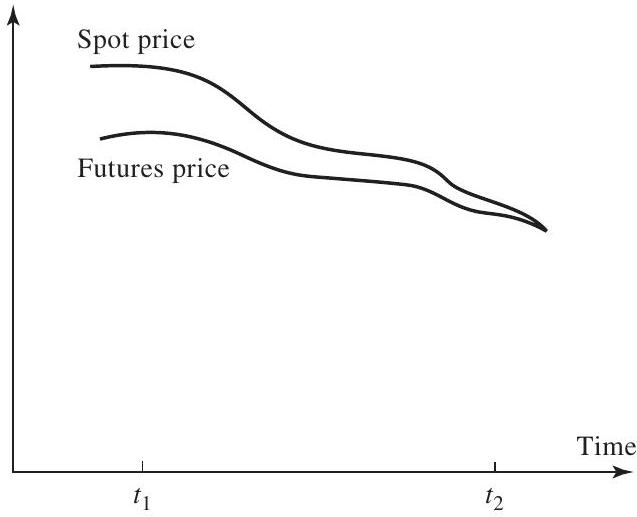
\includegraphics[width=\linewidth]{da7d1f4c-f02d-4245-82cc-df26ce412cbf-076_517_637_1628_455.jpg}
\caption{Spot and futures prices usually move together, but the gap between them
can change before convergence. That changing gap is the basis risk.}
\end{marginfigure}

\subsection{Effective Price in a Short Hedge}

Suppose a firm will sell the asset at time $t_2$. It enters a short futures
position at time $t_1$ at futures price $F_1$ and closes it at $F_2$. The spot
price at $t_2$ is $S_2$. The effective sale price is
\[
    S_2+(F_1-F_2).
\]
Using $b_2=S_2-F_2$, this becomes
\[
    S_2+F_1-F_2=F_1+b_2.
\]

The initial futures price $F_1$ is known at hedge initiation. The final basis
$b_2$ is not known. Therefore the hedge locks in $F_1$ plus an uncertain basis.

\begin{exmp}[Short hedge with basis risk]
A grain producer shorts futures at $F_1=6.20$ dollars per bushel. At harvest,
the local cash price is $S_2=5.85$ and the futures price is $F_2=5.95$. The
final basis is
\[
    b_2=5.85-5.95=-0.10.
\]
The effective sale price is
\[
    F_1+b_2=6.20-0.10=6.10.
\]
Equivalently, the physical sale gives 5.85 and the short futures gain is
$6.20-5.95=0.25$, so the effective price is 6.10.
\end{exmp}

\subsection{Effective Price in a Long Hedge}

Suppose a firm will buy the asset at time $t_2$. It enters a long futures
position at $F_1$ and closes it at $F_2$. The effective purchase price is
\[
    S_2-(F_2-F_1)=F_1+b_2.
\]
Again, the uncertainty is the final basis.

\begin{exmp}[Long hedge with basis risk]
A manufacturer goes long copper futures at $F_1=3.70$. When the hedge is closed,
the physical copper price is $S_2=3.92$ and the futures price is $F_2=3.88$. The
final basis is
\[
    b_2=3.92-3.88=0.04.
\]
The effective purchase price is
\[
    F_1+b_2=3.70+0.04=3.74.
\]
The physical purchase is more expensive than 3.70 because the final basis is
positive.
\end{exmp}

\subsection{Basis Strengthening and Weakening}

The basis strengthens when it increases. It weakens when it decreases.

\begin{tabular}{@{}p{0.25\linewidth}p{0.29\linewidth}p{0.29\linewidth}@{}}
\toprule
Basis movement & Short hedge & Long hedge \\
\midrule
Basis strengthens & improves effective sale price & worsens effective purchase
price \\
Basis weakens & worsens effective sale price & improves effective purchase
price \\
\bottomrule
\end{tabular}

\subsection{Sources of Basis Risk}

Basis risk arises when:
\begin{itemize}
    \item the asset being hedged is not exactly the futures underlying;
    \item the hedge date does not match the futures delivery date;
    \item the delivery location or grade differs from the firm's physical
    exposure;
    \item local supply-demand conditions move cash prices differently from
    exchange futures prices;
    \item the hedge has to be rolled from one contract into another.
\end{itemize}

\begin{boxD}
\textbf{Contract choice.} A common rule is to choose a delivery month as close as
possible to, but later than, the hedge expiration date. The rule must be balanced
against liquidity and delivery-risk concerns.
\end{boxD}

\section{Cross Hedging}

\subsection{When Cross Hedging Is Needed}

A cross hedge uses a futures contract on one asset to hedge exposure to another
asset. It is used when no liquid futures contract exists for the exact exposure.

\begin{exmp}[Jet fuel and heating oil]
An airline wants to hedge jet fuel. If the jet-fuel futures market is illiquid,
the airline might use heating-oil futures because the two prices are strongly
related. The hedge is imperfect because the jet-fuel spread over heating oil can
change.
\end{exmp}

If $S_2$ is the price of the asset being hedged and $S_2^*$ is the spot price of
the asset underlying the futures contract, the final basis can be decomposed as
\[
    S_2-F_2=(S_2-S_2^*)+(S_2^*-F_2).
\]
The first term is the difference between the two assets. The second is the basis
for the futures underlying itself.

\subsection{Minimum-Variance Hedge Ratio}

Let $\Delta S$ be the change in the spot price of the asset being hedged over
the hedge horizon. Let $\Delta F$ be the change in the futures price. If the
hedger uses hedge ratio $h$, a short hedge has change
\[
    \Delta V=\Delta S-h\Delta F.
\]
The variance of the hedged position is
\[
    \Var(\Delta V)
    =
    \sigma_S^2+h^2\sigma_F^2-2h\Cov(\Delta S,\Delta F).
\]
Differentiate with respect to $h$ and set the derivative equal to zero:
\[
    2h\sigma_F^2-2\Cov(\Delta S,\Delta F)=0.
\]
Thus the minimum-variance hedge ratio is
\[
    h^*
    =
    \frac{\Cov(\Delta S,\Delta F)}{\Var(\Delta F)}
    =
    \rho\frac{\sigma_S}{\sigma_F},
\]
where $\rho$ is the correlation between $\Delta S$ and $\Delta F$.

\begin{figure}
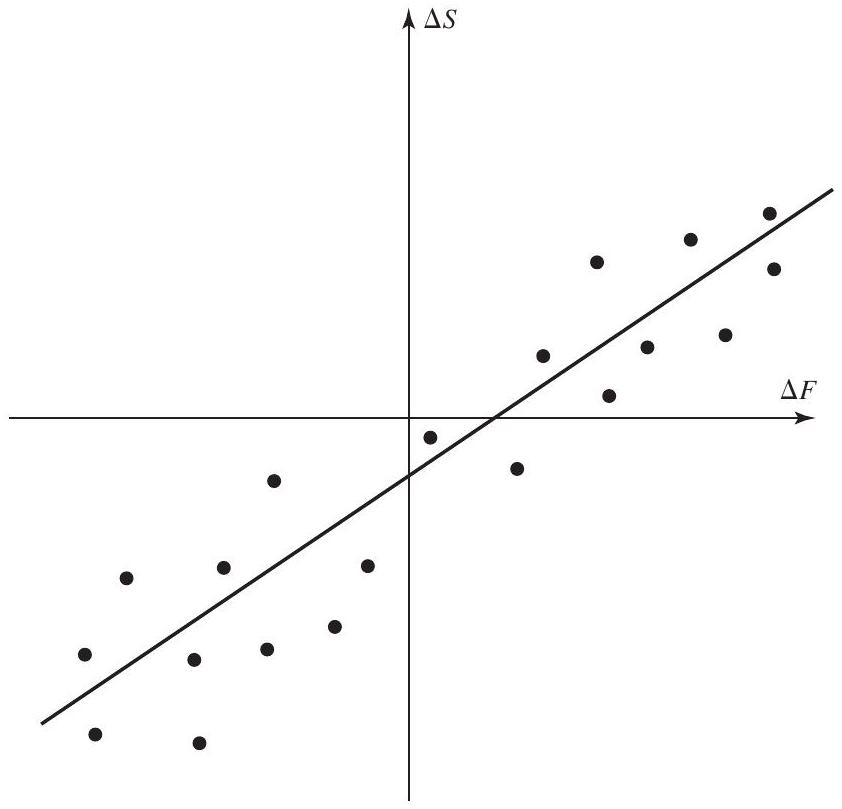
\includegraphics[width=0.48\linewidth]{da7d1f4c-f02d-4245-82cc-df26ce412cbf-080_809_842_1412_453.jpg}
\hfill
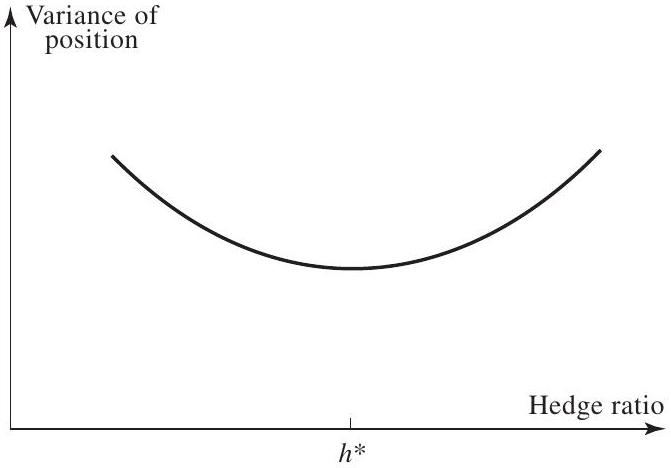
\includegraphics[width=0.48\linewidth]{da7d1f4c-f02d-4245-82cc-df26ce412cbf-081_468_671_339_371.jpg}
\caption{The minimum-variance hedge ratio can be estimated as a regression
slope. The resulting hedge variance is minimized at $h^*$.}
\end{figure}

\begin{boxD}
\textbf{Regression interpretation.} The hedge ratio $h^*$ is the slope in a
regression of spot-price changes on futures-price changes:
\[
    \Delta S=a+h^*\Delta F+\varepsilon.
\]
The hedge effectiveness is the fraction of variance removed by the hedge. In the
simple regression setting it is $R^2=\rho^2$.
\end{boxD}

\subsection{Number of Contracts}

Let $Q_A$ be the size of the exposure and $Q_F$ the size of one futures contract.
The optimal number of contracts is
\[
    N^*=h^*\frac{Q_A}{Q_F}.
\]
If the exposure and futures contract are measured by value rather than physical
quantity, use
\[
    N^*=h^*\frac{V_A}{V_F},
\]
where $V_A$ is the value of the exposure and $V_F$ is the value of one futures
contract.

\begin{exmp}[Cross hedge ratio]
An airline estimates that monthly jet-fuel price changes have standard deviation
$0.18$ dollars per gallon, heating-oil futures price changes have standard
deviation $0.15$, and the correlation is $0.80$. The minimum-variance hedge
ratio is
\[
    h^*=0.80\frac{0.18}{0.15}=0.96.
\]
The airline should hedge 96\% of its physical quantity using heating-oil futures.
The hedge ratio is below or above one depending on relative volatilities and
correlation; it is not mechanically one.
\end{exmp}

\begin{exmp}[Optimal number of contracts]
The airline wants to hedge 3 million gallons of jet fuel. Each heating-oil
futures contract covers 42,000 gallons. With $h^*=0.96$,
\[
    N^*
    =
    0.96\frac{3{,}000{,}000}{42{,}000}
    \approx
    68.57.
\]
The airline would choose 68 or 69 contracts, then consider liquidity,
transaction costs, and whether the hedge should be split across maturities.
\end{exmp}

\subsection{Percentage-Change Hedge Ratios}

Sometimes the regression uses percentage price changes rather than dollar price
changes. If $\hat{h}$ is the slope from percentage changes, then the contract
count should be based on values:
\[
    N^*=\hat{h}\frac{V_A}{V_F}.
\]
This is useful for equity-index hedging, where beta is naturally defined using
returns.

\section{Stock Index Futures and Beta Hedging}

\subsection{Index Futures}

A stock index futures contract gives exposure to a diversified stock index. The
contract value is
\[
    V_F = \text{futures price}\times \text{contract multiplier}.
\]
For example, if an index futures price is 5,200 and the multiplier is USD 50,
one contract has notional value
\[
    5{,}200\times 50=\$260{,}000.
\]

\subsection{Hedging an Equity Portfolio}

If a portfolio mirrors the index, the hedge ratio is approximately one. If the
portfolio has beta $\beta$ relative to the index, the number of contracts to
short is
\[
    N^*=\beta\frac{V_A}{V_F}.
\]

\begin{exmp}[Equity portfolio hedge]
A portfolio is worth USD 40 million and has beta 1.25 relative to an index. The
index futures price is 4,000 and the contract multiplier is USD 250. One
contract has notional value
\[
    V_F=4{,}000\times 250=\$1{,}000{,}000.
\]
The number of contracts required to hedge market risk is
\[
    N^*=1.25\frac{40{,}000{,}000}{1{,}000{,}000}=50.
\]
The portfolio manager shorts 50 futures contracts.
\end{exmp}

\subsection{Changing Portfolio Beta}

Futures can also change, rather than eliminate, market exposure. If the current
portfolio beta is $\beta$ and the target beta is $\beta^*$, then
\[
    N^*=(\beta-\beta^*)\frac{V_A}{V_F}.
\]
If $N^*>0$, short futures. If $N^*<0$, go long futures.

\begin{exmp}[Reducing beta without selling stocks]
A manager has a USD 25 million portfolio with beta 1.40 and wants beta 0.80 for
the next month. Each index futures contract has notional value USD 250,000. The
number of contracts is
\[
    N^*=(1.40-0.80)\frac{25{,}000{,}000}{250{,}000}
    =
    60.
\]
The manager shorts 60 contracts.
\end{exmp}

\begin{exmp}[Increasing beta]
A manager has a USD 10 million portfolio with beta 0.70 and wants beta 1.10. One
futures contract has notional value USD 200,000:
\[
    N^*=(0.70-1.10)\frac{10{,}000{,}000}{200{,}000}
    =
    -20.
\]
The negative sign means the manager should go long 20 contracts.
\end{exmp}

\subsection{Reasons to Use Index Futures}

Index futures can:
\begin{itemize}
    \item temporarily reduce market exposure without selling the underlying
    stocks;
    \item equitize cash during portfolio transitions;
    \item change beta quickly and cheaply;
    \item separate stock selection from market timing.
\end{itemize}

\begin{boxF}
\textbf{Residual risk.} A beta hedge removes exposure to broad market moves only
approximately. The portfolio can still underperform because of stock selection,
sector tilts, changing beta, dividends, liquidity, and futures basis risk.
\end{boxF}

\section{Stack-and-Roll Hedging}

\subsection{The Problem}

Sometimes the exposure lasts longer than the liquid futures contracts available.
The firm then hedges with a nearby contract and rolls the hedge forward as the
nearby contract approaches maturity. This is called \emph{stack and roll}.

\begin{exmp}[Rolling a short hedge]
An oil producer wants to hedge sales over the next 18 months, but the most
liquid futures contracts are in the first six months. The firm may short nearby
contracts, close them as they approach maturity, and open new short positions in
later contracts. The hedge is repeatedly rolled forward.
\end{exmp}

\subsection{Roll Risk}

Rolling creates risk because the contract being closed and the new contract
being opened may have changed in relative price. If the term structure moves
unfavorably, the firm can suffer large cash-flow losses even when the long-run
economics of the hedge are defensible.

\begin{boxF}
\textbf{Risk-management lesson.} A stack-and-roll hedge can transform price risk
into liquidity and funding risk. Daily settlement matters because losses on the
futures position require cash before the physical exposure generates offsetting
cash flows.
\end{boxF}

\section{Forward Prices for Investment Assets}

\subsection{Investment Assets and Consumption Assets}

An \emph{investment asset} is held by many investors primarily for investment
purposes. Examples include stocks, bonds, gold, and silver. A \emph{consumption
asset} is held primarily for use in production or consumption. Examples include
copper, oil, natural gas, wheat, and electricity.

This distinction matters because investment assets can usually be priced by
cash-and-carry arbitrage. Consumption assets can have convenience benefits from
physical ownership that are not captured by a futures contract.

\subsection{Assumptions}

The standard no-arbitrage formulas assume:
\begin{itemize}
    \item no transaction costs or taxes;
    \item borrowing and lending at the same risk-free rate;
    \item ability to short sell when needed;
    \item known income, storage costs, and interest rates;
    \item no default risk.
\end{itemize}
These assumptions are deliberately strong. They identify the clean benchmark.

\subsection{No Income}

For a non-income-paying investment asset, the no-arbitrage forward price is
\[
    F_0=S_0e^{rT}.
\]

\begin{exmp}[Forward price with no income]
A non-dividend-paying stock has price $S_0=80$, the continuously compounded
risk-free rate is $r=4\%$, and maturity is $T=0.75$ years. The forward price is
\[
    F_0=80e^{0.04\times 0.75}=80e^{0.03}\approx 82.44.
\]
\end{exmp}

\begin{exmp}[Cash-and-carry arbitrage]
Suppose the same stock has a quoted forward price of 85. The no-arbitrage price
is 82.44, so the forward is expensive. A trader can:
\begin{enumerate}
    \item borrow 80;
    \item buy the stock;
    \item short the forward at 85.
\end{enumerate}
At maturity, deliver the stock into the forward, receive 85, and repay
\[
    80e^{0.03}=82.44.
\]
The locked-in profit is
\[
    85-82.44=2.56.
\]
\end{exmp}

\begin{exmp}[Reverse cash-and-carry arbitrage]
If the quoted forward price is 81, the forward is cheap. A trader can short the
stock, invest the proceeds, and enter a long forward. At maturity, the investment
is worth 82.44. The trader buys the stock through the forward for 81 and returns
it to close the short sale. The profit is
\[
    82.44-81=1.44.
\]
\end{exmp}

\subsection{Known Income}

If the asset provides known income with present value $I$ during the life of the
forward, the forward price is
\[
    F_0=(S_0-I)e^{rT}.
\]
The income lowers the forward price because the forward buyer does not receive
income paid before delivery.

\begin{exmp}[Forward price with known cash income]
A stock price is 100. It will pay a known dividend of 3 in six months. The
one-year continuously compounded risk-free rate is 5\%. The present value of the
dividend is
\[
    I=3e^{-0.05\times 0.5}\approx 2.93.
\]
The one-year forward price is
\[
    F_0=(100-2.93)e^{0.05}\approx 102.05.
\]
\end{exmp}

\subsection{Known Yield}

If the asset provides a known continuous yield $q$, the forward price is
\[
    F_0=S_0e^{(r-q)T}.
\]
Stock indices and foreign currencies are often modeled this way. For a stock
index, $q$ is the dividend yield. For a foreign currency, $q$ is the foreign
risk-free rate.

\begin{marginfigure}
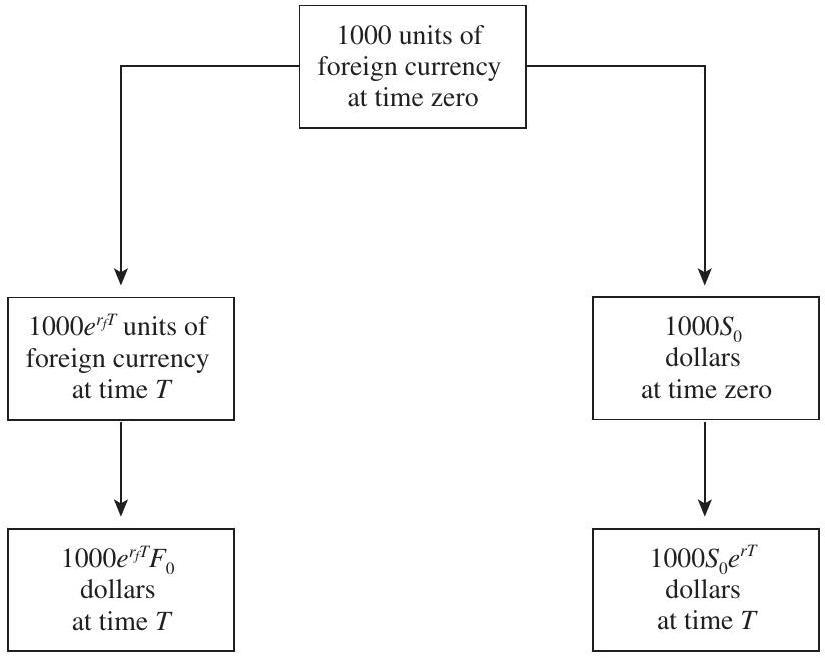
\includegraphics[width=\linewidth]{da7d1f4c-f02d-4245-82cc-df26ce412cbf-138_658_825_423_455.jpg}
\caption{A foreign currency can be treated like an asset with a yield: foreign
interest is the benefit from holding the currency.}
\end{marginfigure}

\begin{exmp}[Index futures price]
An index is at 3,500. The risk-free rate is 4\%, the dividend yield is 1.5\%,
and maturity is four months. With continuous compounding,
\[
    F_0=3{,}500e^{(0.04-0.015)(4/12)}
    =
    3{,}500e^{0.008333}
    \approx 3{,}529.29.
\]
\end{exmp}

\subsection{Value of an Existing Forward Contract}

The delivery price $K$ is fixed in an existing forward contract. The current
forward price $F_0$ is the delivery price that would make a new contract have
zero value. For a long forward with maturity $T$,
\[
    f=(F_0-K)e^{-rT}.
\]

For a non-income-paying asset, this is equivalent to
\[
    f=S_0-Ke^{-rT}.
\]
With known income,
\[
    f=S_0-I-Ke^{-rT}.
\]
With known yield,
\[
    f=S_0e^{-qT}-Ke^{-rT}.
\]

\begin{exmp}[Forward contract value after initiation]
A trader is long a one-year forward with delivery price $K=50$. Six months
later, the current six-month forward price for the asset is $F_0=54$ and the
six-month risk-free rate is 4\% continuously compounded. The value of the long
forward is
\[
    f=(54-50)e^{-0.04\times 0.5}
    =
    4e^{-0.02}
    \approx 3.92.
\]
The contract is valuable because it allows the trader to buy at 50 when the
current forward price is 54.
\end{exmp}

\section{Futures Prices Versus Forward Prices}

For many purposes, especially with deterministic interest rates, futures and
forward prices are treated as equal. Daily settlement is the key difference.
Futures gains and losses are realized every day, while forward gains and losses
accumulate until maturity.

When interest rates are uncertain:
\begin{itemize}
    \item if futures prices tend to rise when interest rates rise, long futures
    gains can be reinvested at high rates, making futures prices tend to exceed
    forward prices;
    \item if futures prices tend to fall when interest rates rise, long futures
    losses occur when financing is expensive, making futures prices tend to be
    below forward prices.
\end{itemize}

\begin{boxD}
\textbf{Practical convention.} For short-dated contracts and many classroom
applications, we use the same pricing formula for forwards and futures. The
distinction matters more when interest rates are volatile and strongly
correlated with futures price changes.
\end{boxD}

\section{Commodity Forward and Futures Prices}

\subsection{Storage Costs}

Storage costs act like negative income. If the present value of storage costs is
$U$, the forward price for an investment commodity is
\[
    F_0=(S_0+U)e^{rT}.
\]
If storage costs are proportional to the spot price at continuous rate $u$, then
\[
    F_0=S_0e^{(r+u)T}.
\]

\begin{exmp}[Commodity with fixed storage costs]
Silver is at USD 25 per ounce. Storage costs have present value USD 0.40 per
ounce over the life of a nine-month contract. The risk-free rate is 5\%. The
forward price is
\[
    F_0=(25+0.40)e^{0.05\times 0.75}
    \approx 26.37.
\]
\end{exmp}

\begin{exmp}[Commodity with proportional storage costs]
A commodity spot price is 60. The risk-free rate is 4\%, storage costs are 2\%
per year proportional to the spot price, and maturity is one year. Then
\[
    F_0=60e^{(0.04+0.02)}\approx 63.71.
\]
\end{exmp}

\subsection{Convenience Yield}

For a consumption commodity, physical ownership can provide benefits that a
futures contract does not provide:
\begin{itemize}
    \item ability to keep a production process running;
    \item ability to profit from temporary shortages;
    \item avoiding disruption from supply-chain problems;
    \item meeting customer demand immediately.
\end{itemize}
These benefits are summarized by the \emph{convenience yield}.

With proportional storage cost $u$ and convenience yield $y$, the common
cost-of-carry expression is
\[
    F_0=S_0e^{(r+u-y)T}.
\]

\begin{exmp}[Convenience yield]
Oil has spot price 80. The risk-free rate is 5\%, storage costs are 1\% per year
of spot value, and the convenience yield is 4\%. For a six-month contract,
\[
    F_0=80e^{(0.05+0.01-0.04)(0.5)}
    =
    80e^{0.01}
    \approx 80.80.
\]
Without convenience yield, the price would be
\[
    80e^{(0.05+0.01)(0.5)}\approx 82.44.
\]
The convenience yield reduces the futures price because physical ownership has a
benefit.
\end{exmp}

\subsection{Investment Commodities Versus Consumption Commodities}

For an investment commodity such as gold, arbitrage can often pin down the
forward price from spot price, interest rates, and storage costs. For a
consumption commodity such as oil or copper, arbitrage usually gives an upper
bound rather than an exact price:
\[
    F_0\leq (S_0+U)e^{rT}.
\]
If the futures price were above this bound, traders could buy and store the
commodity and short futures. If the futures price is below the bound, the
reverse trade may be impossible because holders of the physical commodity may
not be willing to sell inventory and give up convenience benefits.

\begin{boxF}
\textbf{Important distinction.} A low futures price for a consumption commodity
does not automatically imply arbitrage. The missing asset is the convenience
benefit from physical inventory.
\end{boxF}

\subsection{Cost of Carry}

The cost of carry is the cost of financing and storing the asset, minus income
earned on the asset. For an investment asset,
\[
    F_0=S_0e^{cT},
\]
where $c$ is the cost of carry.

For a consumption commodity with convenience yield $y$,
\[
    F_0=S_0e^{(c-y)T}.
\]

\subsection{Contango and Backwardation}

A futures curve is in \emph{contango} when futures prices tend to rise with
maturity. It is in \emph{backwardation} when futures prices tend to fall with
maturity.

Contango is often associated with financing and storage costs exceeding
convenience yield. Backwardation is often associated with high convenience yield,
scarcity, or strong current demand for the physical commodity.

\begin{exmp}[Reading a futures curve]
Suppose spot oil is 82, the three-month futures price is 81, and the one-year
futures price is 77. The curve is downward sloping. One interpretation is that
near-term physical oil has a high convenience yield: inventory is valuable today
because users want immediate access to the commodity.
\end{exmp}

\section{Expected Future Spot Prices}

\subsection{Futures Price Is Not Usually an Unbiased Forecast}

It is tempting to say that the futures price equals the expected future spot
price. This is not generally correct. Futures prices are pricing objects, not
pure forecasts.

Let $k$ be the required expected return on the underlying asset. A simple
relationship is
\[
    F_0=\E(S_T)e^{(r-k)T}.
\]
Therefore:

\begin{tabular}{@{}lll@{}}
\toprule
Systematic risk & Relation between $k$ and $r$ & Implication \\
\midrule
No systematic risk & $k=r$ & $F_0=\E(S_T)$ \\
Positive systematic risk & $k>r$ & $F_0<\E(S_T)$ \\
Negative systematic risk & $k<r$ & $F_0>\E(S_T)$ \\
\bottomrule
\end{tabular}

\begin{exmp}[Positive systematic risk]
A stock index has positive systematic risk, so investors require an expected
return above the risk-free rate. The futures price can be below the expected
future index level even though there is no arbitrage. The gap compensates
investors for bearing market risk.
\end{exmp}

\subsection{Normal Backwardation and Contango}

Keynes and Hicks emphasized hedging pressure. If producers are natural short
hedgers and speculators take the long side, speculators may require a positive
expected return. In that case the futures price may be below the expected future
spot price. This is often called normal backwardation.

If consumers are natural long hedgers and speculators take the short side, the
reverse can occur: the futures price may exceed the expected future spot price.

\begin{boxD}
\textbf{Do not confuse terms.} Backwardation and contango describe the shape of
the futures curve across maturities. Normal backwardation and normal contango
describe the relation between a futures price and the expected future spot price.
\end{boxD}

\section{Commodity Behavior from Chapter 35}

\subsection{Agricultural Commodities}

Agricultural commodities often have:
\begin{itemize}
    \item strong seasonality;
    \item weather-driven supply shocks;
    \item high volatility before harvest;
    \item storage limits and quality deterioration;
    \item jumps when information about crop size changes.
\end{itemize}

\subsection{Metals}

Precious metals such as gold and silver are closer to investment assets because
they are widely held for investment. Industrial metals such as copper are closer
to consumption assets because users value physical inventory for production.

\subsection{Energy Products}

Energy markets are central for hedging because both prices and quantities are
uncertain.
\begin{itemize}
    \item Crude oil can be stored, but storage capacity and location matter.
    \item Natural gas demand is seasonal and weather-sensitive.
    \item Electricity is difficult to store economically, so spot prices can
    spike sharply when demand or supply surprises occur.
\end{itemize}

\begin{exmp}[Electricity and spikes]
If a heat wave increases air-conditioning demand while generation capacity is
tight, electricity spot prices can jump. A futures or forward contract hedges
average price over a delivery period, but it may not perfectly hedge operational
exposure to hourly spikes unless the contract is designed for that load shape.
\end{exmp}

\subsection{Mean Reversion and Seasonality}

Commodity prices often display mean reversion: high prices encourage supply and
discourage demand, while low prices discourage production and encourage demand.
Seasonality arises when supply or demand follows the calendar.

\begin{figure}
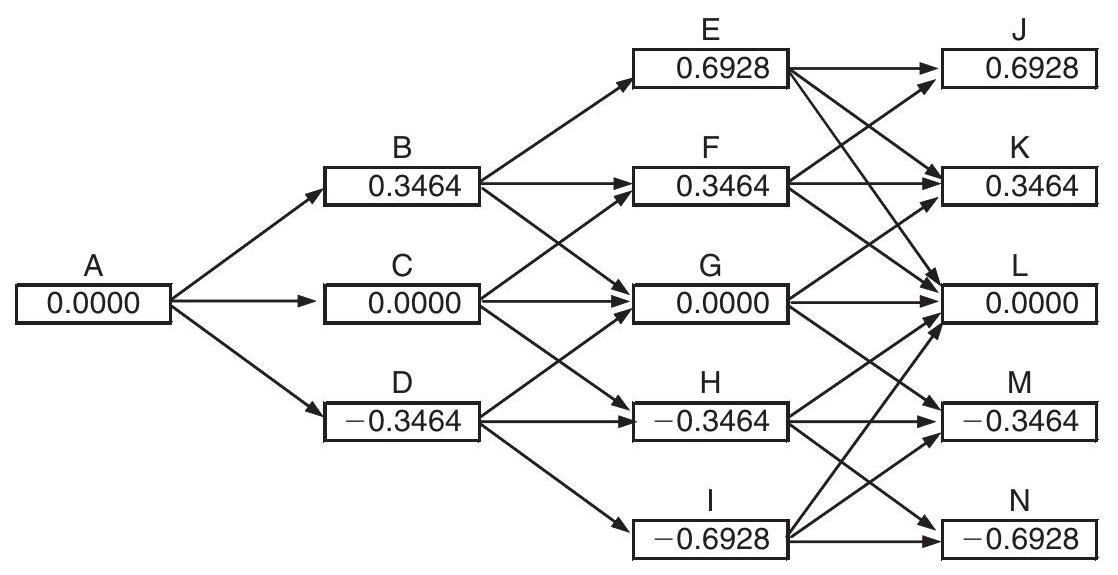
\includegraphics[width=0.32\linewidth]{da7d1f4c-f02d-4245-82cc-df26ce412cbf-791_575_1118_422_360.jpg}
\hfill
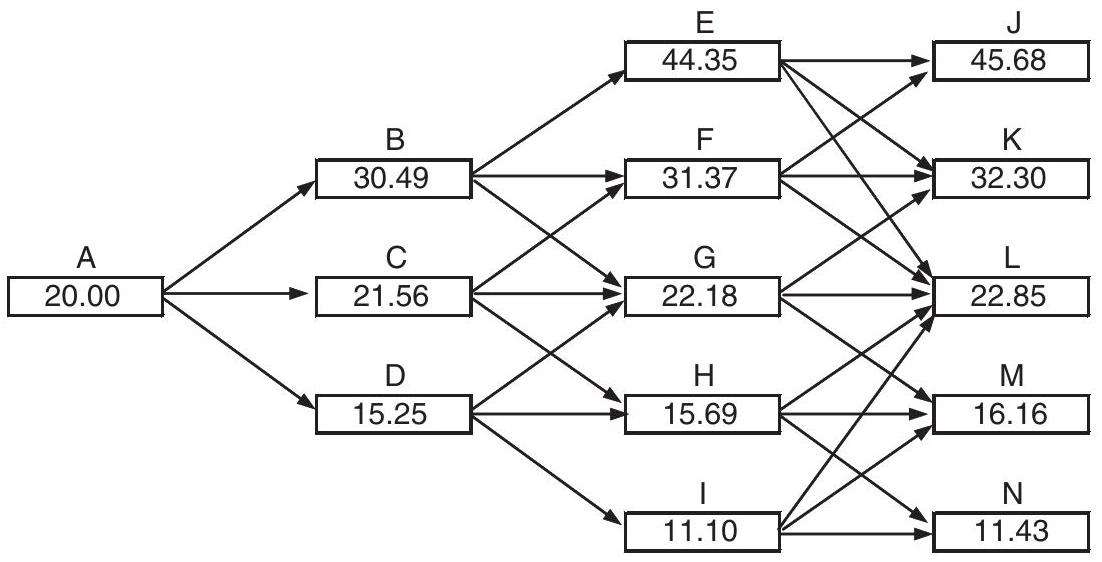
\includegraphics[width=0.32\linewidth]{da7d1f4c-f02d-4245-82cc-df26ce412cbf-792_562_1102_1460_455.jpg}
\hfill
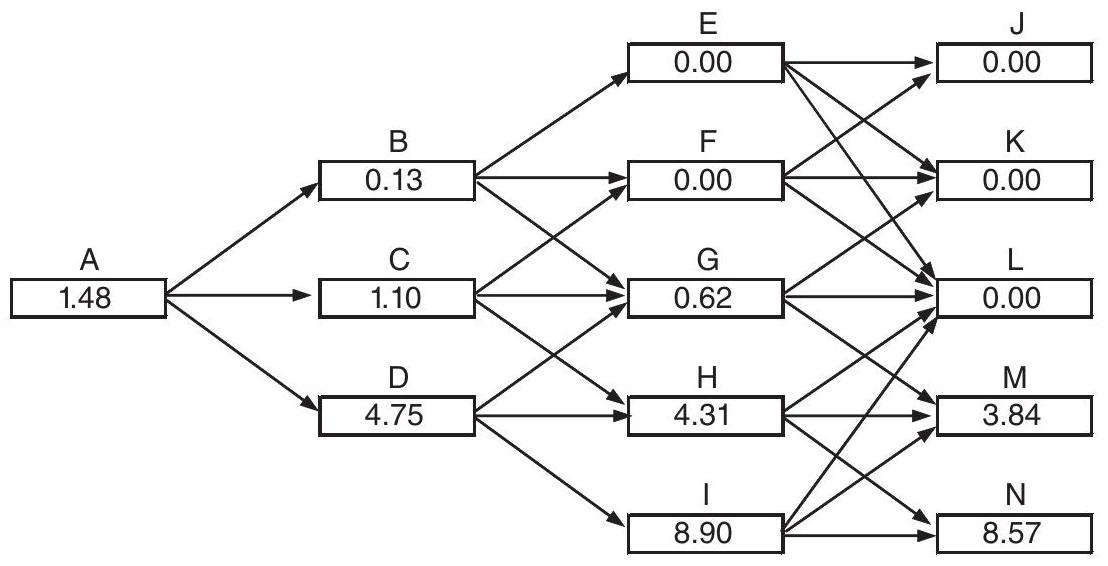
\includegraphics[width=0.32\linewidth]{da7d1f4c-f02d-4245-82cc-df26ce412cbf-793_566_1108_378_365.jpg}
\caption{Commodity derivative models often use trees calibrated to futures
prices. The economic inputs are not only volatility, but also term structure,
seasonality, mean reversion, and convenience yield.}
\end{figure}

\begin{boxF}
\textbf{Modeling caution.} Equity models often begin with geometric Brownian
motion. Commodity models often need storage, seasonality, mean reversion, jumps,
and convenience yields. The economic structure of the underlying asset matters.
\end{boxF}

\section{Worked Problems}

\begin{exmp}[Short hedge effective price]
A firm shorts futures at 48.00 to hedge a sale. When the hedge is closed, the
spot price is 46.80 and the futures price is 47.10. The basis is
\[
    b_2=46.80-47.10=-0.30.
\]
The effective sale price is
\[
    F_1+b_2=48.00-0.30=47.70.
\]
\end{exmp}

\begin{exmp}[Long hedge effective price]
A firm goes long futures at 112.50. At the purchase date, the spot price is
118.00 and the futures price is 117.20. The final basis is
\[
    b_2=118.00-117.20=0.80.
\]
The effective purchase price is
\[
    112.50+0.80=113.30.
\]
\end{exmp}

\begin{exmp}[Minimum-variance hedge ratio]
Spot price changes have standard deviation 2.4, futures price changes have
standard deviation 3.0, and their correlation is 0.75:
\[
    h^*=0.75\frac{2.4}{3.0}=0.60.
\]
If the exposure is 120,000 units and each futures contract is for 10,000 units,
\[
    N^*=0.60\frac{120{,}000}{10{,}000}=7.2.
\]
The hedger would use about 7 contracts.
\end{exmp}

\begin{exmp}[Equity hedge]
A portfolio is worth EUR 18 million and has beta 0.9. Index futures are quoted
at 6,000 with multiplier EUR 10. One contract has value EUR 60,000. The number
of contracts for a full market hedge is
\[
    N^*=0.9\frac{18{,}000{,}000}{60{,}000}=270.
\]
The manager shorts 270 contracts.
\end{exmp}

\begin{exmp}[Forward price with known yield]
An index is 1,200, the risk-free rate is 3.5\%, the dividend yield is 2.0\%, and
maturity is nine months. Then
\[
    F_0=1{,}200e^{(0.035-0.020)(0.75)}
    =
    1{,}200e^{0.01125}
    \approx 1{,}213.58.
\]
\end{exmp}

\begin{exmp}[Value of a forward on an income-paying asset]
A stock is 60. A dividend of 1.50 will be paid in three months. A long forward
with six months remaining has delivery price 58. The continuously compounded
risk-free rate is 4\%. The present value of the dividend is
\[
    I=1.50e^{-0.04(0.25)}\approx 1.485.
\]
The value of the long forward is
\[
    f=S_0-I-Ke^{-rT}
    =
    60-1.485-58e^{-0.04(0.5)}
    \approx 1.66.
\]
\end{exmp}

\begin{exmp}[Storage cost and convenience yield]
A commodity spot price is 45. Financing cost is 4\%, proportional storage cost
is 3\%, and convenience yield is 2\%. For a one-year contract,
\[
    F_0=45e^{(0.04+0.03-0.02)}
    =
    45e^{0.05}
    \approx 47.31.
\]
\end{exmp}

\begin{exmp}[Futures price and expected spot]
A commodity has expected future spot price $\E(S_T)=100$, risk-free rate
$r=3\%$, required return $k=7\%$, and maturity $T=1$. Then
\[
    F_0=100e^{(0.03-0.07)}
    =
    100e^{-0.04}
    \approx 96.08.
\]
The futures price is below the expected future spot price because the asset has
positive systematic risk.
\end{exmp}

\section{Checklist for Students}

After this lecture you should be able to:
\begin{itemize}
    \item decide whether a short hedge or long hedge is appropriate;
    \item compute futures gains and losses for hedging examples;
    \item define the basis as $S_t-F_t$ and compute effective hedge prices;
    \item explain why basis risk remains after hedging;
    \item decompose basis risk in a cross hedge;
    \item derive and use $h^*=\rho\sigma_S/\sigma_F$;
    \item compute the optimal number of futures contracts;
    \item hedge an equity portfolio with stock-index futures;
    \item change a portfolio beta using futures;
    \item explain stack-and-roll hedging and roll risk;
    \item derive $F_0=S_0e^{rT}$ by no-arbitrage;
    \item price forwards with known income and known yield;
    \item value an existing forward contract;
    \item distinguish investment assets and consumption assets;
    \item use storage costs and convenience yield in commodity pricing;
    \item distinguish futures prices from expected future spot prices.
\end{itemize}

\section{Practice Questions}

\begin{enumerate}
    \item A firm will sell 2 million gallons of a commodity in three months. The
    futures contract size is 50,000 gallons. Should the firm go long or short?
    How many contracts are needed for a one-to-one hedge?
    \item A buyer will purchase 100,000 units in six months. It goes long
    futures at 18.40. At the purchase date the spot price is 20.10 and the
    futures price is 19.90. Compute the final basis and effective purchase
    price.
    \item A seller shorts futures at 72. The final spot price is 70 and the
    final futures price is 69.50. Compute the effective sale price.
    \item Explain why basis strengthening helps a short hedger but hurts a long
    hedger.
    \item Spot-price changes have standard deviation 5, futures-price changes
    have standard deviation 4, and the correlation is 0.64. Compute the
    minimum-variance hedge ratio and hedge effectiveness.
    \item A firm has exposure to 400,000 units. Each futures contract covers
    20,000 units. If $h^*=0.80$, compute the optimal number of contracts.
    \item A portfolio is worth USD 75 million and has beta 1.10. Index futures
    are quoted at 4,800 with multiplier 250. How many contracts should be
    shorted to hedge market exposure?
    \item The same portfolio manager wants to reduce beta from 1.10 to 0.60.
    How many contracts should be used?
    \item A non-dividend-paying stock has $S_0=42$, $r=5\%$, and $T=0.5$.
    Compute the forward price.
    \item If the quoted forward price in the previous question is 44.50,
    describe the arbitrage.
    \item A stock is 90 and will pay a known dividend with present value 2. The
    risk-free rate is 4\% and maturity is one year. Compute the forward price.
    \item An index is 2,000, the risk-free rate is 3\%, the dividend yield is
    1.2\%, and maturity is six months. Compute the futures price.
    \item A long forward has delivery price 100. The current forward price for
    the remaining maturity is 108, the risk-free rate is 5\%, and remaining
    maturity is one year. Compute the value of the long forward.
    \item A commodity has spot price 35 and storage costs with present value 1.2.
    The risk-free rate is 6\% and maturity is nine months. Compute the
    no-arbitrage forward price for an investment commodity.
    \item A commodity has spot price 70, financing cost 4\%, storage cost 2\%,
    convenience yield 5\%, and maturity one year. Compute the futures price
    using the cost-of-carry formula.
    \item Explain why the reverse cash-and-carry arbitrage may fail for a
    consumption commodity.
    \item Distinguish contango from normal contango.
    \item If $\E(S_T)=50$, $r=3\%$, $k=1\%$, and $T=1$, compute $F_0$ and
    explain the sign of the risk premium.
    \item Give two reasons electricity prices can be more volatile than crude
    oil prices.
    \item Explain how weather can create both price risk and volume risk for an
    energy producer.
\end{enumerate}

\end{document}
